\documentclass[a4paper,10pt,twoside]{book}
\usepackage{amd}

% %--------------------------------------------------------------------------
% %         General Setting
% %--------------------------------------------------------------------------

\graphicspath{{Images/}{../Images/}} %Path of figures
\setkeys{Gin}{width=0.85\textwidth} %Size of figures
\setlength{\cftbeforechapskip}{3pt} %space between items in toc
\setlength{\parindent}{0.5cm} % Idk
% Theorem System
% The following boxes are provided:
%   Definition:     \defn 
%   Theorem:        \thm 
%   Lemma:          \lem
%   Corollary:      \cor
%   Proposition:    \prop   
%   Claim:          \clm
%   Fact:           \fact
%   Proof:          \pf
%   Example:        \ex
%   Remark:         \rmk (sentence), \rmkb (block)
% Suffix
%   r:              Allow Theorem/Definition to be referenced, e.g. thmr
%   p:              Add a short proof block for Lemma, Corollary, Proposition or Claim, e.g. lemp
%                   For theorems, use \pf for proof blocks

% ======= Real examples : 

% \defn{Definition Name}{
%     A defintion.
% }

% \thmr{Theorem Name}{mybigthm}{
%     A theorem.
% }

% \lem{Lemma Name}{
%     A lemma.
% }

% \fact{
%     A fact.
% }

% \cor{
%     A corollary.
% }

% \prop{
%     A proposition.
% }

% \clmp{}{
%     A claim.
% }{
%     A reference to Theorem~\ref{thm:mybigthm}
% }

% \pf{
%    proof.

% \ex{
%     some examples. 
% }

% \rmk{
%     Some remark.
% }

% \rmkb{
%     Some more remark.
% }

\usepackage{xcolor}

% Define custom colors
\definecolor{defscol}{HTML}{ecd8d7} %For definitions
\definecolor{asumscol}{HTML}{ecd8d7} %For Assumptions

\definecolor{rmkscol}{HTML}{313160} %For remarks
\definecolor{exmscol}{HTML}{e04b52} %For examples

\definecolor{lemscol}{HTML}{2c3943} %For Lemmes
\definecolor{thmscol}{HTML}{595765} %For Theorems
\definecolor{prpscol}{HTML}{9c98b1} %For proposition
\definecolor{corscol}{HTML}{dfd9fd} %For corrolaries

\definecolor{clmscol}{HTML}{165c58} %For claims
\definecolor{facscol}{HTML}{28a8a1} %For facts



% ============================
% Definition
% ============================
\newtcbtheorem[number within=section]{mydefinition}{Definition}
{
    enhanced,
    frame hidden,
    titlerule=0mm,
    toptitle=1mm,
    bottomtitle=1mm,
    fonttitle=\bfseries\large,
    coltitle=black,
    colbacktitle=defscol!40!white,
    colback=defscol!20!white,
}{defn}

\NewDocumentCommand{\defn}{m+m}{
    \begin{mydefinition}{#1}{}
        #2
    \end{mydefinition}
}

\NewDocumentCommand{\defnr}{mm+m}{
    \begin{mydefinition}{#1}{#2}
        #3
    \end{mydefinition}
}

% ============================
% Assumption
% ============================
\newtcbtheorem[use counter from=mydefinition]{myassumption}{Assumption}
{
    enhanced,
    frame hidden,
    titlerule=0mm,
    toptitle=1mm,
    bottomtitle=1mm,
    fonttitle=\bfseries\large,
    coltitle=black,
    colbacktitle=asumscol!40!white,
    colback=asumscol!20!white,
}{asum}

\NewDocumentCommand{\asum}{m+m}{
    \begin{myassumption}{#1}{}
        #2
    \end{myassumption}
}

\NewDocumentCommand{\asumr}{mm+m}{
    \begin{myassumption}{#1}{#2}
        #3
    \end{myassumption}
}

% ============================
% Theorem
% ============================

\newtcbtheorem[use counter from=mydefinition]{mytheorem}{Theorem}
{
    enhanced,
    frame hidden,
    titlerule=0mm,
    toptitle=1mm,
    bottomtitle=1mm,
    fonttitle=\bfseries\large,
    coltitle=black,
    colbacktitle=thmscol!40!white,
    colback=thmscol!20!white,
}{thm}

\NewDocumentCommand{\thm}{m+m}{
    \begin{mytheorem}{#1}{}
        #2
    \end{mytheorem}
}

\NewDocumentCommand{\thmr}{mm+m}{
    \begin{mytheorem}{#1}{#2}
        #3
    \end{mytheorem}
}

\newenvironment{thmpf}{
	{\noindent{\it \textbf{Proof for Theorem.}}}
	\tcolorbox[blanker,breakable,left=5mm,parbox=false,
    before upper={\parindent15pt},
    after skip=10pt,
	borderline west={1mm}{0pt}{thmscol!40!white}]
}{
    \textcolor{thmscol!40!white}{\hbox{}\nobreak\hfill$\blacksquare$} 
    \endtcolorbox
}

\NewDocumentCommand{\thmp}{m+m+m}{
    \begin{mytheorem}{#1}{}
        #2
    \end{mytheorem}

    \begin{thmpf}
        #3
    \end{thmpf}
}

% ============================
% Lemma
% ============================

\newtcbtheorem[use counter from=mydefinition]{mylemma}{Lemma}
{
    enhanced,
    frame hidden,
    titlerule=0mm,
    toptitle=1mm,
    bottomtitle=1mm,
    fonttitle=\bfseries\large,
    coltitle=black,
    colbacktitle=lemscol!40!white,
    colback=lemscol!20!white,
}{lem}

\NewDocumentCommand{\lem}{m+m}{
    \begin{mylemma}{#1}{}
        #2
    \end{mylemma}
}

\newenvironment{lempf}{
	{\noindent{\it \textbf{Proof for Lemma}}}
	\tcolorbox[blanker,breakable,left=5mm,parbox=false,
    before upper={\parindent15pt},
    after skip=10pt,
	borderline west={1mm}{0pt}{lemscol!40!white}]
}{
    \textcolor{lemscol!40!white}{\hbox{}\nobreak\hfill$\blacksquare$} 
    \endtcolorbox
}

\NewDocumentCommand{\lemp}{m+m+m}{
    \begin{mylemma}{#1}{}
        #2
    \end{mylemma}

    \begin{lempf}
        #3
    \end{lempf}
}

% ============================
% Corollary
% ============================

\newtcbtheorem[use counter from=mydefinition]{mycorollary}{Corollary}
{
    enhanced,
    frame hidden,
    titlerule=0mm,
    toptitle=1mm,
    bottomtitle=1mm,
    fonttitle=\bfseries\large,
    coltitle=black,
    colbacktitle=corscol!40!white,
    colback=corscol!20!white,
}{cor}

\NewDocumentCommand{\cor}{+m}{
    \begin{mycorollary}{}{}
        #1
    \end{mycorollary}
}

\newenvironment{corpf}{
	{\noindent{\it \textbf{Proof for Corollary.}}}
	\tcolorbox[blanker,breakable,left=5mm,parbox=false,
    before upper={\parindent15pt},
    after skip=10pt,
	borderline west={1mm}{0pt}{corscol!40!white}]
}{
    \textcolor{corscol!40!white}{\hbox{}\nobreak\hfill$\blacksquare$} 
    \endtcolorbox
}

\NewDocumentCommand{\corp}{m+m+m}{
    \begin{mycorollary}{}{}
        #1
    \end{mycorollary}

    \begin{corpf}
        #2
    \end{corpf}
}

% ============================
% Proposition
% ============================

\newtcbtheorem[use counter from=mydefinition]{myproposition}{Proposition}
{
    enhanced,
    frame hidden,
    titlerule=0mm,
    toptitle=1mm,
    bottomtitle=1mm,
    fonttitle=\bfseries\large,
    coltitle=black,
    colbacktitle=prpscol!30!white,
    colback=prpscol!20!white,
}{prop}

\NewDocumentCommand{\prop}{+m}{
    \begin{myproposition}{}{}
        #1
    \end{myproposition}
}

\newenvironment{proppf}{
	{\noindent{\it \textbf{Proof for Proposition.}}}
	\tcolorbox[blanker,breakable,left=5mm,parbox=false,
    before upper={\parindent15pt},
    after skip=10pt,
	borderline west={1mm}{0pt}{prpscol!40!white}]
}{
    \textcolor{prpscol!40!white}{\hbox{}\nobreak\hfill$\blacksquare$} 
    \endtcolorbox
}



\NewDocumentCommand{\propp}{+m+m}{
    \begin{myproposition}{}{}
        #1
    \end{myproposition}

    \begin{proppf}
        #2
    \end{proppf}
}

% ============================
% Claim
% ============================

\newtcbtheorem[use counter from=mydefinition]{myclaim}{Claim}
{
    enhanced,
    frame hidden,
    titlerule=0mm,
    toptitle=1mm,
    bottomtitle=1mm,
    fonttitle=\bfseries\large,
    coltitle=black,
    colbacktitle=clmscol!40!white,
    colback=clmscol!20!white,
}{clm}

\NewDocumentCommand{\clm}{m+m}{
    \begin{myclaim*}{#1}{}
        #2
    \end{myclaim*}
}

\newenvironment{clmpf}{
	{\noindent{\it \textbf{Proof for Claim.}}}
	\tcolorbox[blanker,breakable,left=5mm,parbox=false,
    before upper={\parindent15pt},
    after skip=10pt,
	borderline west={1mm}{0pt}{clmscol!40!white}]
}{
    \textcolor{clmscol!40!white}{\hbox{}\nobreak\hfill$\blacksquare$} 
    \endtcolorbox
}

\NewDocumentCommand{\clmp}{m+m+m}{
    \begin{myclaim*}{#1}{}
        #2
    \end{myclaim*}

    \begin{clmpf}
        #3
    \end{clmpf}
}

% ============================
% Fact
% ============================

\newtcbtheorem[use counter from=mydefinition]{myfact}{Fact}
{
    enhanced,
    frame hidden,
    titlerule=0mm,
    toptitle=1mm,
    bottomtitle=1mm,
    fonttitle=\bfseries\large,
    coltitle=black,
    colbacktitle=facscol!40!white,
    colback=facscol!20!white,
}{fact}

\NewDocumentCommand{\fact}{+m}{
    \begin{myfact}{}{}
        #1
    \end{myfact}
}

% ============================
% Proof
% ============================

\NewDocumentCommand{\pf}{+m}{
    \begin{proof}
        [\noindent\textbf{Proof.}]
        #1
    \end{proof}
}

% ============================
% Example
% ============================


\newenvironment{myexample}{
    \tcolorbox[blanker,breakable,left=5mm,parbox=false,
    before upper={\parindent15pt},
    after skip=10pt,
	borderline west={1mm}{0pt}{clmscol!40!white}]
}{
    \textcolor{clmscol!40!white}{\hbox{}\nobreak\hfill$\blacksquare$} 
    \endtcolorbox
}

\NewDocumentCommand{\exm}{m+m}{
    \begin{myexample}
	{\noindent{\it \textbf{Example : #1 }}}\\ 
        #2
    \end{myexample}
}


% ============================
% Remark
% ============================


\NewDocumentCommand{\rmk}{+m}{
    {\it \color{rmkscol!40!white}#1}
}

\newenvironment{remark}{
    \par
    \vspace{5pt}
    \begin{minipage}{\textwidth}
        {\par\noindent{\textbf{Remark.}}}
        \tcolorbox[blanker,breakable,left=5mm,
        before skip=10pt,after skip=10pt,
        borderline west={1mm}{0pt}{rmkscol!20!white}]
}{
        \endtcolorbox
    \end{minipage}
    \vspace{5pt}
}

\NewDocumentCommand{\rmkb}{+m}{
    \begin{remark}
        #1
    \end{remark}
}













% % Old styles hh 

% %--------------------------------------------------------------------------
% % 		THEOREMES STYLE
% %--------------------------------------------------------------------------

% %-------		DEFINITION 		-------	
% \newcounter{defo}[chapter]
% \newenvironment{defi}[1]{\refstepcounter{defo} 
% \begin{tcolorbox}[colback=yellow!20!white,colframe=yellow!15!black,title= \textbf{Définition \thechapter \ $\blacklozenge$ \thedefo \ | #1}]}{\end{tcolorbox}}

% %-------		THEOREME 		-------	
% \newcounter{th}[chapter]
% \newenvironment{thm}[1]{\refstepcounter{th}
% \begin{tcolorbox}[colback=mycolor!10,colframe=mycolor!10!black!80,title=\textbf{ Théorème \thechapter \ $\blacklozenge$ \theth \ | #1}]}{\end{tcolorbox}}

% %-------		PROPOSITION 		-------	
% \newcounter{prop}[chapter]
% \newenvironment{propt}[1]{\refstepcounter{prop}
% \begin{tcolorbox}[colback=mycolor!5,colframe=mycolor!10!linkscolor!80 ,title=\textbf{ Proposition \thechapter \ $\blacklozenge$ \theprop \ | #1}]}{\end{tcolorbox}}

% %-------		COROLLAIRE		-------
% \newcounter{cor}[chapter]
% \newenvironment{corr}[1]{\refstepcounter{cor}
% \begin{tcolorbox}[colback=mycolor!2,colframe=mycolor!10!linkscolor!40 ,title= Corolaire \thechapter \ $\blacklozenge$ \thecor \ | #1]}{\end{tcolorbox}}

% %-------		LEMME			-------
% \newcounter{lem}[chapter]
% \newenvironment{lemme}[1]{\refstepcounter{lem}
% \begin{tcolorbox}[colback=mycolor!10!blue!2,colframe=mycolor!50!blue!30,title=\textbf{Lemme \thechapter \ $\blacklozenge$ \thelem \ | #1}]}{\end{tcolorbox}}

% %-------		METHODE 			-------
% \newcounter{met}[chapter]
% \newenvironment{meth}[1]{\refstepcounter{met}
% \begin{tcolorbox}
% [enhanced jigsaw,breakable,pad at break*=1mm,
%  colback=red!20!white,boxrule=0pt,frame hidden,
%  borderline west={1.5mm}{-2mm}{red}] \color{red}
% {\textbf{Méthode \thechapter \ $\blacklozenge$ \themet \ | #1} } \color{black} \\ } {\end{tcolorbox}}

% %-------		REMARQUE 			-------
% \newcommand{\NB}[1]{
% \ \\
% \begin{tabular}{p{0.05\textwidth}p{0.80\textwidth}}
% \hline
% \vspace{-0.1cm} \includegraphics[scale=0.03]{./system/IDEA.png} & 	#1\\
% \hline
% \end{tabular}
% \ 
% \newline \ \newline
%  }

% %-------		EXEMPLE  		-------
% \newenvironment{exm}{ \begin{tcolorbox}
% [enhanced jigsaw,breakable,pad at break*=1mm,
%  colback=cyan!20!white,boxrule=0pt,frame hidden,
%  borderline west={1.5mm}{-2mm}{cyan}] \color{cyan}
% {\textbf{Exemple} } \color{black} \\ } {\end{tcolorbox}}
  % Theorems styles and colors
\usepackage[english]{babel} %Language
\usepackage{framed}

\setlist[itemize]{itemsep=5pt} % Adjust the length as needed
\setlist[enumerate]{itemsep=5pt} % Adjust the length as needed



% \usepackage{lmodern} %  Latin Modern font
% \usepackage{newtxtext,newtxmath}




% %--------------------------------------------------------------------------
% %         General Informations
% %--------------------------------------------------------------------------
\newcommand{\BigTitle}{
    Compilers: Principles, Techniques, \& Tools
    }

\newcommand{\LittleTitle}{
    By Alfred V. Aho et all
    }

    
\begin{document}

% %--------------------------------------------------------------------------
% %         First pages 
% %--------------------------------------------------------------------------
\newgeometry{top=8cm,bottom=.5in,left=2cm,right=2cm}
\subfile{files/0.0.0.titlepage}
\restoregeometry
\thispagestyle{empty}
\setcounter{page}{0}
\tableofcontents
\thispagestyle{empty}
\setcounter{page}{0}

% %--------------------------------------------------------------------------
% %         Core of the document 
% %--------------------------------------------------------------------------
\chapter{Introduction}

The world as we know it depends on programming languages, because all the software running on all the computers was written in some programming language. But, before a program can be run, it first must be translated into a form in which it can be executed by a computer.

The software systems that do this translation are called \textit{compilers}.

\section{Language Processors}

Simply stated, a compiler is a program that can read a program in one language--the \textit{source} language--and translate it into an equivalent program in another language--the \textit{target} language.

An \textit{interpreter} is another common kind of language processor.

The task of collecting the source program is sometimes entrusted to a separate program, called a \textit{preprocessor}.

The compiler may produce an assembly-language program as its output, because assembly language is easier to produce as output and is easier to debug. The assembly language is then processed by a program called an \textit{assembler} that produces relocatable machine code as its output.

The \textit{linker} resolves external memory addresses, where the code in one file may refer to a location in another file. The \textit{loader} then puts together all of the executable object files into memory for execution.

\section{The Structure of a Compiler}

Up to this point we have treated a compiler as a single box that maps a source program into a semantically equivalent target program. If we open up this box a little, we see that there are two parts to this mapping: analysis and synthesis.

The \textit{analysis} part breaks up the source program into constituent pieces and imposes a grammatical structure on them. The analysis part also collects information about the source program and stores it in a data structure called a \textit{symbol table}, which is passed along with the intermediate representation to the synthesis part.

The \textit{synthesis} part constructs the desired target program from the intermediate representation and the information in the symbol table. The analysis part is often called the \textit{front end} of the compiler; the synthesis part is the \textit{back end}.

If we examine the compilation process in more detail, we see that it operates as a sequence of \textit{phases}, each of which transforms one representation of the source program to another.

\subsection{Lexical Analysis}

The first phase of a compiler is called \textit{lexical analysis} or \textit{scanning}. The lexical analyzer reads the stream of characters making up the source program and groups the characters into meaningful sequences called \textit{lexemes}. For each lexeme, the lexical analyzer produces as output a \textit{token} of the form $$\langle\textit{token-name, attribute-value}\rangle$$ that is passes on to the subsequent phase, syntax analysis. In the token, the first component \textit{token-name} is an abstract symbol that is used during syntax analysis, and the second component \textit{attribute-value} points to an entry in the symbol table for this token.

\subsection{Syntax Analysis}

The second phase of the compiler is \textit{syntax analysis} or \textit{parsing}. A typical representation is a \textit{syntax tree} in which each interior node represents an operation and the children of the node represent the arguments of the operation.

\subsection{Semantic Analysis}

The \textit{semantic analyzer} uses the syntax tree and the information in the symbol table to check the source program for semantic consistency with the language definition.

An important part of semantic analysis is \textit{type checking}, where the compiler checks that each operator has matching operands.

The language specification may permit some type conversions called \textit{coercions}.

\subsection{Intermediate Code Generation}

We consider an intermediate form called \textit{three-address code}, which consists of a sequence of assembly-like instructions with three operands per instruction.

\subsection{The Grouping of Phases into Passes}

In an implementation, activities from several phases may be grouped together into a \textit{pass} that reads an input file and writes an output file.

\subsection{Compiler-Construction Tools}

Some commonly used compiler-construction tools include
\begin{enumerate}
    \item \textit{Parser generators} that automatically produce syntax analyzers from a grammatical description of a programming language.
    \item \textit{Scanner generators} that produce lexical analyzers from a regular-expression description of the tokens of a language.
    \item \textit{Syntax-directed translation engines} that produce collections of routines for walking a parse tree and generating intermediate code.
    \item \textit{Code-generator generators} that produce a code generator from a collection of rules for translating each operation of the intermediate language into the machine language for a target machine.
    \item \textit{Data-flow analysis engines} that facilitate the gathering of information about how values are transmitted from one part of a program to each other part.
    \item \textit{Compiler-construction toolkits} that provide an integrated set of routines for construction various phases of a compiler.
\end{enumerate}

\section{The Evolution of Programming Language}
\subsection{The Move to Higher-Level Languages}

One classification is by generation. \textit{First-generation languages} are the machine languages, \textit{second-generation} the assembly languages, and \textit{third-generation} the higher-level languages. \textit{Fourth-generation languages} are languages designed for specific applications. The term \textit{fifth-generation language} has been applied to logic- and constraint-based languages.

Another classification of languages uses the term \textit{imperative} for languages in which a program specifies \textit{how} a computation is to be done and \textit{declarative} for languages in which a program specifies \textit{what} computation is to be done.

The term \textit{von Neumann language} is applied to programming languages whose computational model is based on the von Neumann computer architecture.

An \textit{object-oriented language} is one that supports object-oriented programming, a programming style in which a program consists of a collection of objects that interact with one another.

\textit{Scripting languages} are interpreted languages with high-level operators designed for "gluing together" computations.

\section{Applications of Compiler Technology}
\subsection{implementation of High-Level Programming Languages}

A body of compiler optimizations, known as \textit{data-flow optimizations}, has been developed to analyze the flow of data through the program and removes redundancies across these constructs.

Object-oriented programs are different from those written in many other languages, in that they consist of many more, but smaller, procedures (called \textit{methods} in object-oriented terms).

\subsection{Optimizations for Computer Architectures}

Almost all high-performance systems take advantage of the same two basic techniques: \textit{parallelism} and \textit{memory hierarchies}. Parallelism can be found at several levels: at the \textit{instruction level}, where multiple operations are executed simultaneously and at the \textit{processor level}, where different threads of the same application are run on different processors.

\section{Programming Language Basics}
\subsection{The Static/Dynamic Distinction}

If a language uses a policy that allows the compiler to decide an issue, then we say that the language uses a \textit{static} policy or that the issue can be decided at \textit{compile time}. On the other hand, a policy that only allows a decision to be made when we execute the program is said to be a \textit{dynamic policy} or to require a decision at \textit{run time}.

The \textit{scope} of a declaration of $x$ is the region of the program in which uses of $x$ refer to this declaration. A language uses \textit{static scope} or \textit{lexical scope} if it is possible to determine the scope of a declaration by looking only at the program. Otherwise, the language uses \textit{dynamic scope}.

\subsection{Environments and States}

\begin{figure}[htbp]
    \centering
    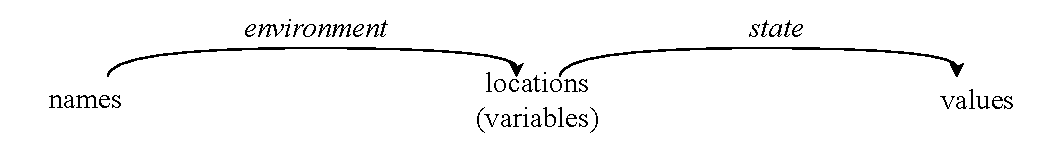
\includegraphics[width=\linewidth]{Figure1 8.pdf}
    \caption{Two-stage mapping from names to values}
    \label{figure:1.8}
\end{figure}

The association of names with locations in memory (the \textit{store}) and then with values can be described by two mappings that change as the program runs:
\begin{enumerate}
    \item The \textit{environment} is a mapping from names to locations in the store.
    \item The \textit{state} is a mapping from locations in store to their values.
\end{enumerate}

The environment and state mappings in Fig.\;\ref{figure:1.8} are dynamic, but there are a few exceptions:
\begin{enumerate}
    \item \textit{Static versus dynamic binding} of names to locations.
    \item \textit{Static versus dynamic binding} of locations to values.
\end{enumerate}

\begin{framed}
\begin{center}
    \textbf{{\large Names, Identifiers, and Variables}}
\end{center}

An \textit{identifier} is a string of characters, typically letters or digits, that refers to (identifies) an entity. Composite names are called \textit{qualified} names.

A \textit{variable} refers to a particular location of the store.
\end{framed}

\subsection{Static Scope and Block Structure}

The scope rules for C are based on program structrue; the scope of a declaration is determined implicitly by where the declaration appears in the program. Later languages also provide explicit control over scopes through the use of keywords like \textbf{public}, \textbf{private} and \textbf{protected}.

A \textit{block} is a grouping of declarations and statements. C uses braces \texttt{\{} and \texttt{\}} to delimit a block; the alternative use of \textbf{begin} and \textbf{end} for the same purpose dates back to Algol.

In C, the syntax of blocks is given by
\begin{enumerate}
    \item One type of statement is a block. Blocks can appear anywhere that other types of statement can appear.
    \item A block is a sequence of declarations followed by a sequence of statements, all surrounded by braces.
\end{enumerate}

Note that this syntax allows blocks to be nested inside each other. This nesting property is referred to as \textit{block structure}.

\subsection{Explicit Access Control}

Through the use of keywords like \textbf{public}, \textbf{private}, and \textbf{protected}, object-oriented languages provide explicit control over access to member names in a superclass. These keywords support \textit{encapsulation} by restricting access.

\subsection{Dynamic Scope}

Technically, any scoping policy is dynamic if it is based on factor(s) that can be known only when the program executes. The term \textit{dynamic scope}, however, usually refers to the following policy: a use of a name $x$ refers to the declaration of $x$ in the most recently called procedure with such a declaration.

\begin{framed}
    \begin{center}
        \textbf{{\large Declarations and Definitions}}
    \end{center}

    In C++, a method is declared in a class definition, by giving the types of the arguments and result of the method (often called the \textit{signature} for the method).
\end{framed}

\subsection{Parameter Passing Mechanisms}

\textit{Actual parameters} (the parameters used in the call of a procedure) are associated with the \textit{formal parameters} (those used in the procedure definition).

\subsubsection{Call-by-Value}

In \textit{call-by-value}, the actual parameter is evaluated (if it is an expression) or copied (if it is a variable).

\subsubsection{Call-by-Reference}

In \textit{call-by-reference}, the address of the actual parameter is passed to the callee as the value of the corresponding formal parameter.

\subsection{Aliasing}

It is possible that two formal parameters can refer to the same location; such variables are said to be \textit{aliases} of one another.

% %--------------------------------------------------------------------------
% %         Bibliographie 
% %--------------------------------------------------------------------------
\end{document}
